\documentclass{beamer}
\usepackage[utf8x]{inputenc}
\usepackage{graphicx}
%
% Choose how your presentation looks.
%
% For more themes, color themes and font themes, see:
% http://deic.uab.es/~iblanes/beamer_gallery/index_by_theme.html
%
\mode<presentation>
{
  \usetheme{NYU}      % or try Darmstadt, Madrid, Warsaw, ...
  \usecolortheme{default} % or try albatross, beaver, crane, ...
  \usefonttheme{default}  % or try serif, structurebold, ...
  \setbeamertemplate{navigation symbols}{}
  \setbeamertemplate{caption}[numbered]
} 

\usepackage[english]{babel}
\usepackage[T1]{fontenc}
\usepackage[utf8x]{inputenc}
\usepackage{gensymb}

\title[]{Control Systems}
\subtitle{Gate Question Presentation}
\author{Ritwik Sahani}
\institute{IITH}



\begin{document}

\begin{frame}
  \titlepage
\end{frame}

\begin{frame}{Question}
\centerline{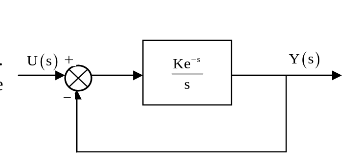
\includegraphics[scale=.5 ]{helpme}}
  Q. Consider the unity feedback control system shown. The value of K the results in the phase margin of system to be 30\degree  is 
  
  Ans: 1.047
  
\end{frame}

\begin{frame}{Definition}
\centerline{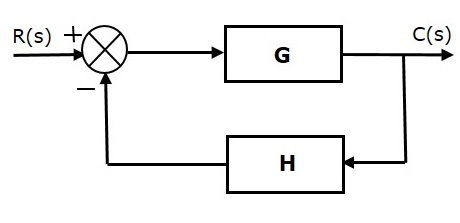
\includegraphics[scale=.5 ]{negative_feedback}}
Phase margin is the difference between phase of G(s)H(s) and -180\degree evaluated at gain crossover frequency ($\omega_{gc}$).

Where $\omega _{gc}$ is defined as the frequency at which magnitude of G(s)H(s) is unity.
\newline\newline
PM = $\phi$ - (-180\degree)  = $\phi$ + 180\degree
\end{frame}

\begin{frame}{Calculation}
In our case H(s) = 1, G(s) = ${Ke^{-s}}/s$ .
\newline
\newline
Put s =  j$\omega$ for frequency domain analysis, and equate |G(j$\omega_{gc}$)|to 1.
\newline
We have,
\newline
\newline
 $|\frac{{Ke^{-j\omega_{gc}}}}{j\omega_{gc}}|$ = 1 \implies $\omega_{gc}$ = K (assuming positive K) \newline\newline

then, $\angle G(j\omega_{gc}$) H(j$\omega_{gc}$) = $\angle \frac{{Ke^{-j\omega_{gc}}}}{j\omega_{gc}}$ =  $\angle \frac{{Ke^{-jK}}}{jK}$  
\newline\newline
\implies -90\degree - K*180/\pi  \quad\quad\quad [=\phi]



\end{frame}
\begin{frame}{Calculation}
PM = 30\degree =  $\phi$ + 180\degree
\newline\newline
On solving, we get K = $\frac{\pi}{3}$  = 1.047
\end{frame}
\begin{frame}{Verification}
\centerline{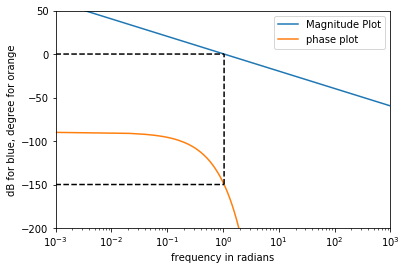
\includegraphics[scale=.75]{graph}}

\end{frame}


\end{document}



